\documentclass[10pt]{article}
\usepackage{multicol} 					% for tables with multiple columns
\usepackage{color} 							% for coloured text
\usepackage{pgfplots} 					% for graphics in latex
\usepackage{tikz} 							% for graphics in latex
\usepackage{amsmath,amssymb,bm,amsthm} % for math symbols and notation
\usepackage{graphicx,epstopdf}	% for figures
\usepackage{pdfpages}						% include pages from another pdf. \includepdf[pages={-}]{myfile.pdf}
\usepackage{fullpage} 					% page layout
\usepackage{hyperref} 					% hyperlinks in text
\usepackage[backend=bibtex,giveninits=true,dateabbrev=true,style=ieee]{biblatex} % for the bibliography 										% all of the packages used in the document
\addbibresource{WSDcurrent.bib}  	% This contains your references
%%%%% This is a file for keeping your macros. Use them whenever possible, so you can change notation on-the-fly. This also helps you use notation more consistently. Annotate so that it is searchable when you inevitably forget the macro for something.

%%%%% vectors, matrices, etc
\newcommand{\Mat}[1]{\begin{bmatrix}#1\end{bmatrix}}	% Matrix detail
\newcommand{\vect}[1]{\bm{\mathrm{#1}}}								% Vector, bolded
\def\omat{\vect{0}} 	% zero matrix
\def\ident{\vect{I}} 	% identity matrix
\newcommand{\norm}[1]{\left\|#1\right\|}
\def\trans{\mathrm{T}}

%%%%% For coloured writing, corrections
\newcommand{\red}[1]{\textcolor{red}{#1}} % red writing

%%%%% Environments
\newcommand{\Item}[1]{\begin{itemize}#1\end{itemize}}			% Itemized list
\newcommand{\Enum}[1]{\begin{enumerate}#1\end{enumerate}}	% Ennumerated list
\newcommand{\aleq}[1]{\begin{align}#1\end{align}} 				% aligned equation, not numbered
\newcommand{\aleqn}[1]{\begin{align*}#1\end{align*}} 			% aligned equation, numbered	

%%%%%% Sets
\def\IR{\mathbb R}					% Real #'s
\def\IC{\mathbb C}					% Complex #'s
\def\IZ{\mathbb Z}					% Integers
\def\IN{\mathbb N}					% Natural #'s

%%%%% References etc...
\newcommand{\fref}[1]{Figure~\ref{#1}} 	% Reference figures
\newcommand{\iref}[1]{Item~\ref{#1}} 		% Reference figures
\newcommand{\tref}[1]{Table~\ref{#1}}		% Reference figures

%%%%% theorems etc...
\newtheorem{Asm}{Assumption}

%%%%% Symbols
\def\done{\tikz\fill[scale=0.4](0,.35) -- (.25,0) -- (1,.7) -- (.25,.15) -- cycle;} % checkmark

%%%%% Signature line
\def\SignatureAndDate{%
    \par\noindent\makebox[1.5in]{\hrulefill} \hfill \makebox[2.5in]{\hrulefill} \hfill \makebox[2in]{\hrulefill}%
    \par\noindent\makebox[1.5in]{Date (day/month/year)} \hfill \makebox[2.5in]{Signature} \hfill \makebox[2in]{Printed name}%
} 							% your macros
\usepackage{float}
\usepackage[ruled,vlined]{algorithm2e}
\usepackage{array}
\usepackage{nicefrac}
\newcolumntype{L}[1]{>{\raggedright\let\newline\\\arraybackslash\hspace{0pt}}m{#1}}


\usepackage{acronym}% heard about a great LaTeX package and thought I'd share. It's the acronym package. It lets you define a macro for each acronym, e.g.\acrodef{uav}[{\sc uav}]{unmanned aerial vehicle}. Then, when you want to use the acronym, you type \ac{uav} for singular and \acp{uav} for plural. The package will figure out when you first use the acronym and introduce it properly.
\usepackage{pdflscape}
\usepackage{comment}
\usepackage{subcaption}

% Theorem environments
\theoremstyle{definition}
\newtheorem{define}{Definition}
\newtheorem{theorem}{Theorem}
\newtheorem{lemma}{Lemma}
\newtheorem{problem}{Problem}
\newtheorem{assumption}{Assumption}
\newtheorem{case}{Case}
\newtheorem{pf}{Proof}
\newtheorem{preliminaries}{Preliminaries}
\newtheorem{cor}{Corollary}
\newtheorem{property}{Property}
\newtheorem{remark}{Remark}
\newtheorem{prop}{Proposition}

% Macro for \Autoref (takes in multiple references)
\makeatletter
\newcommand\Autoref[1]{\@first@ref#1,@}
\def\@throw@dot#1.#2@{#1}% discard everything after the dot
\def\@set@refname#1{%    % set \@refname to autoefname+s using \getrefbykeydefault
	\edef\@tmp{\getrefbykeydefault{#1}{anchor}{}}%
	\xdef\@tmp{\expandafter\@throw@dot\@tmp.@}%
	\ltx@IfUndefined{\@tmp autorefnameplural}%
	{\def\@refname{\@nameuse{\@tmp autorefname}s}}%
	{\def\@refname{\@nameuse{\@tmp autorefnameplural}}}%
}
\def\@first@ref#1,#2{%
	\ifx#2@\autoref{#1}\let\@nextref\@gobble% only one ref, revert to normal \autoref
	\else%
	\@set@refname{#1}%  set \@refname to autoref name
	\@refname~\ref{#1}% add autoefname and first reference
	\let\@nextref\@next@ref% push processing to \@next@ref
	\fi%
	\@nextref#2%
}
\def\@next@ref#1,#2{%
	\ifx#2@ and~\ref{#1}\let\@nextref\@gobble% at end: print and+\ref and stop
	\else, \ref{#1}% print  ,+\ref and continue
	\fi%
	\@nextref#2%
}
\newcommand{\card}{\mbox{card}} % cardinality
\newcommand{\bcard}{\overline{\mbox{card}}} % block cardinality
\newcommand{\block}{\mbox{block}} % block partition operator
\newcommand{\Bfrak}{\mathfrak{B}} % block
\newcommand{\Gfrak}{\mathfrak{G}} % graph
\newcommand{\Scal}{\mathcal{S}} % structure
\newcommand{\Chat}{\widehat{C}} % Chat
\newcommand{\Ahat}{\widehat{A}} % Ahat
\newcommand{\Bhat}{\widehat{B}} % Bhat
\newcommand{\Dhat}{\widehat{D}} % Dhat
\newcommand{\GfrakC}{\Gfrak^c} % graph for Chat
\newcommand{\BfrakC}{\Bfrak^c} % block for Chat
\newcommand{\Bfrakx}{\Bfrak^A} % block for A
\newcommand{\Bfraky}{\Bfrak^B} % block for B
\newcommand{\Bfrakz}{\Bfrak^C} % block for C
\newcommand{\bb}[1]{\mathbb{#1}} % double bar R
\newcommand{\I}{\mathbf{I}} % bold I
\newcommand{\mbf}[1]{\mathbf{#1}} % bold
\newcommand{\bmat}[1]{\begin{bmatrix} #1 \end{bmatrix}} % bracketed matrix
\newcommand{\Blue}[1]{\textcolor{blue}{#1}} % blue text
\newcommand{\Red}[1]{\textcolor{red}{#1}} % blue text
\newcommand{\Hcal}{\mathcal{H}} % curly H
\newcommand{\cone}{\mbox{cone}} % cone
\newcommand{\excone}{\mbox{excone}} % excone
\newcommand{\xhat}{\hat{\mathbf{x}}} % xhat
\newcommand{\A}{\mathbf{A}} % bold A
\newcommand{\B}{\mathbf{B}} % bold B
\newcommand{\C}{\mathbf{C}} % bold C
\newcommand{\D}{\mathbf{D}} % bold D
\newcommand{\U}{\mathbf{U}} % bold D
\newcommand{\x}{\mathbf{x}} % bold x
\newcommand{\bu}{\mathbf{u}} % bold u
\newcommand{\y}{\mathbf{y}} % bold y
\newcommand{\w}{\mathbf{w}} % bold w
\newcommand{\z}{\mathbf{z}} % bold z
\newcommand{\bP}{\mathbf{P}} % bold P
\newcommand{\Q}{\mathbf{Q}} % bold Q
\newcommand{\tr}{\mbox{tr}} % trace
\newcommand{\K}{\mbf{K}} % bold K
\newcommand{\E}{\mbf{E}} % bold E
\newcommand{\bS}{\mbf{S}} % bold S
\newcommand{\R}{\mbf{R}}
\newcommand{\F}{\mbf{F}}
\newcommand{\bH}{\mbf{H}}
\newcommand{\Z}{\mbf{Z}}
\newcommand{\T}{\mbf{T}}
\newcommand{\Qt}{\widetilde{\Q}}
\newcommand{\Kt}{\widetilde{\K}}
\newcommand{\dQ}{\delta\Q}
\newcommand{\dK}{\delta\K}
\newcommand{\He}{\mbox{He}}
\newcommand{\M}{\mbf{M}}
\newcommand{\bL}{\mbf{L}}
\newcommand{\W}{\mbf{W}}
\newcommand{\V}{\mbf{V}}
\newcommand{\Pt}{\widetilde{\mbf{P}}}
\newcommand{\dP}{\delta\mbf{P}}
\newcommand{\dPt}{\delta\Pt}
\newcommand{\X}{\mbf{X}}
\newcommand{\yhat}{\hat{\mbf{y}}}
\newcommand{\zero}{\mbf{0}}
\newcommand{\At}{\widetilde{\A}}
\newcommand{\Bt}{\widetilde{\B}}
\newcommand{\Ct}{\widetilde{\C}}
\newcommand{\Qtc}{\widetilde{\Q}_c}
\newcommand{\Ptc}{\widetilde{\bP}_c}
\newcommand{\St}{\widetilde{\bS}}
\newcommand{\Stc}{\widetilde{\bS}_c}
\newcommand{\Rt}{\widetilde{\R}}
\newcommand{\Rtc}{\widetilde{\R}_c}
\newcommand{\one}{\mbf{1}}
\newcommand{\G}{\mbf{G}}
\newcommand{\st}{\mbox{s.t.}}
\newcommand{\bc}{\mbf{c}}
\newcommand{\e}{\mbf{e}}
\newcommand{\br}{\mbf{r}}
\newcommand{\cs}{\mbox{cs}}
\newcommand{\mbar}{{\bar m}}
\newcommand{\nbar}{{\bar n}}
\newcommand{\step}{\hspace{3mm}}
\newcommand{\Phat}{\widehat{P}}
\newcommand{\Shat}{\widehat{S}}
\newcommand{\Qhat}{\widehat{Q}}
\newcommand{\Rhat}{\widehat{R}}
\newcommand{\uhat}{\widehat{\bu}}
\newcommand{\Y}{\mbf{Y}}
\newcommand{\Pbar}{\bar{\bP}}
\newcommand{\dPbar}{\delta\bar{\bP}}
\newcommand{\dF}{\delta\F}
\newcommand{\dS}{\delta\bS}
\newcommand{\Hinf}{\Hcal_\infty}
\newcommand{\Qbar}{\bar{Q}}
\newcommand{\Sbar}{\bar{S}}
\newcommand{\Rbar}{\bar{R}}
\newcommand{\Xcal}{\mathcal{X}}
\newcommand{\Ycal}{\mathcal{Y}}
\newcommand{\Ncal}{\mathcal{N}}
\newcommand{\Qcal}{\mathcal{Q}}
\newcommand{\Rcal}{\mathcal{R}}
\newcommand{\Lcal}{\mathcal{L}}
\newcommand{\Gcal}{\mathcal{G}}
\newcommand{\Htwo}{{\Hcal_2}}
\newcommand{\Acal}{\mathcal{A}}
\newcommand{\Bcal}{\mathcal{B}}
\newcommand{\Ccal}{\mathcal{C}}
\newcommand{\Tcal}{{\mathcal{T}}}
\newcommand{\Ocal}{{\mathcal{O}}}
\newcommand{\Nbar}{{\bar{N}}}
\newcommand{\Space}{\hspace{2mm}}
\newcommand{\aseq}{\overset{a.s.}{=}}
\newcommand{\xb}{\bar{x}}
\newcommand{\expect}[1]{\mathbb{E}[#1]}
\newcommand{\Expect}[1]{\mathbb{E}\Big[#1\Big]}
\newcommand{\prob}[1]{\mathbb{P}(#1)}
\newcommand{\Prob}[1]{\mathbb{P}\Big(#1\Big)}


\usepackage[margin=0.5in]{geometry}
\begin{document}
	
	
	\title{Drone Network Decomposition}
	\author{Ethan LoCicero}
	\date{November 7, 2024}
	\maketitle

	% =========================================================

Our controller converts roll, pitch, yaw and/or their rates to torques in the same dimensions. From Brogliado, we know that Lagrangian systems are passive from torque inputs to angular velocity outputs\footnote{I never found this result written out, but Leila references it all the time, and I didn't look that hard because even taking it as true, there were more pressing things to solve. But we need to find it eventually.}. That means from torques to roll, pitch, and yaw rates, the drone must be passive. If we ignore motor dynamics and say that the controller can provide torque actuation exactly, and then we could design the controller to be strictly passive to ensure stability. This is visualized in \autoref{fig:DroneComposite}.

\begin{figure}
	\centering
	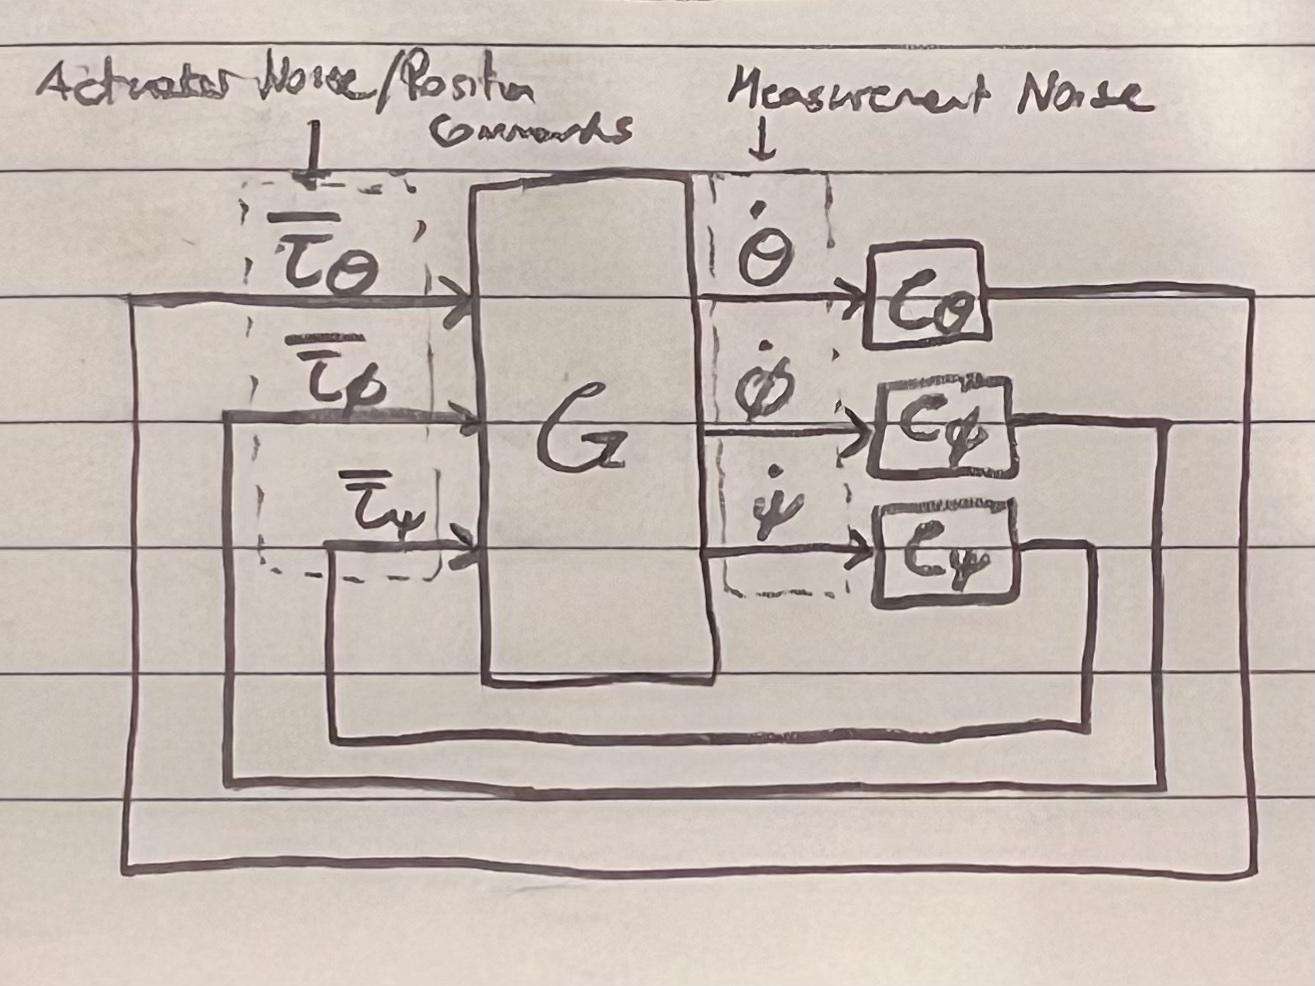
\includegraphics[width=.5\textwidth]{DroneComposite}
	\caption{Drone in feedback with controller, neglecting motor dynamics. The overlines on $\tau$'s indicate the commanded torque. Roll, pitch, and yaw are $\theta$, $\phi$, and $\psi$, respectively, and $\mathcal{G}$ is the drone dynamics. (Note: where it says ``Actuator noise/Position commands" and ``Measurement noise", it means those exogenous signals are added there).}\label{fig:DroneComposite}
\end{figure}

However, the motors introduce non-trivial dynamics that must be accounted for, and these likely violate passivity. In reality, the drone can be decomposed as visualized in \autoref{fig:DroneNetwork}. Here, we see that the controller mappings are the same, but the commanded torques, $\overline{\tau}_{(\cdot)}$ (and commanded lift force, $\overline{F}_L$) are converted to squares of commanded rotor speeds using the matrix $\Gamma^{-1}$, where
\begin{align*}
	\Gamma = \bmat{k & k & k & k \\ 0 & lk & 0 & -lk \\ lk & 0 & -lk & 0 \\ -b & b & -b & b}
\end{align*}
The motor dynamics, $\mathcal{M}$, then convert the commanded motor speeds, $\overline{\omega}$, to actual motor speeds, $\omega$, before $\Omega$ coverts these motor speeds squared back to actual torques (and lift force) that effect the drone frame dynamics, $\mathcal{G}$. (Notice, the lift force doesn't effect roll, pitch, and yaw, so it's excluded from the drone inputs, and x,y,z position and their rates are also currently excluded). The motor dynamics are given by 
\begin{align*}
	v &= Ri + L\frac{di}{dt} + k_e \omega \\
	J\dot{\omega} &= -k_Ti - b\omega^2,
\end{align*}
where $v$ is voltage, $i$ is current, $\omega$ is rotor speed, $R$ is resistance, $L$ is inductance, $k_e$ is the back-EMF coefficient, $k_T$ is the torque constant, $J$ is the inertia, and $b$ is the rotor drag constant. The voltage is restricted as $v \in [0,v_\mathrm{max}(t)]$, where $v_\mathrm{max}(t) \leq 12.6$. This is because the minimum voltage applied to the motors is $0$, and the maximum is the instantaneous maximum voltage of the battery, which can be charged to at most $12.6V$. We want the voltage to equal the demanded rotor speed when the motors are at equilibrium, which is satisfied by $v = \frac{Rb}{k_T}\overline{\omega}^2 + k_e\overline{\omega}$, where $\overline{w}$ is the commanded rotor speed (as opposed to actual). Substituting the relation for voltage and letting $x^T = [i \; \omega]$, $u = \overline{\omega}^2$, and $y = \omega^2$, we have
\begin{align*}
	\dot{x} &= \bmat{-\frac{R}{L} & -\frac{k_e}{L} \\ \frac{k_T}{J} & 0 }x + \bmat{0 & 0 \\ 0 & -\frac{b}{J} }x^2 + \frac{1}{L}\mathrm{sat}_{[0,v_{\mathrm{max}}(t)]}\left(\bmat{\frac{Rb}{k_T} \\ 0}u + \bmat{k_e \\ 0}\sqrt{u}\right) \\
	y &=  \bmat{0 & 1}x^2.
\end{align*}
The matrices $\Gamma$ and $\Gamma^{-1}$ are linear, so this network fits into the framework of Vidyasagar's Network Dissipativity Theorem (VNDT). As before, the drone frame can be viewed as passive since it is a Lagrangian system, provided we consider the control inputs to be the roll pitch and yaw rates. (If the control inputs are just the angles themselves, we would need a different dissipativity characterization of the frame). The motor dynamics have nonlinear input and output functions, so we will need a clever way of analyzing them, possibly using Reza, Amy, and Frank's triangulation method, or possibly using Ethan's data methods.

\begin{figure}
	\centering
	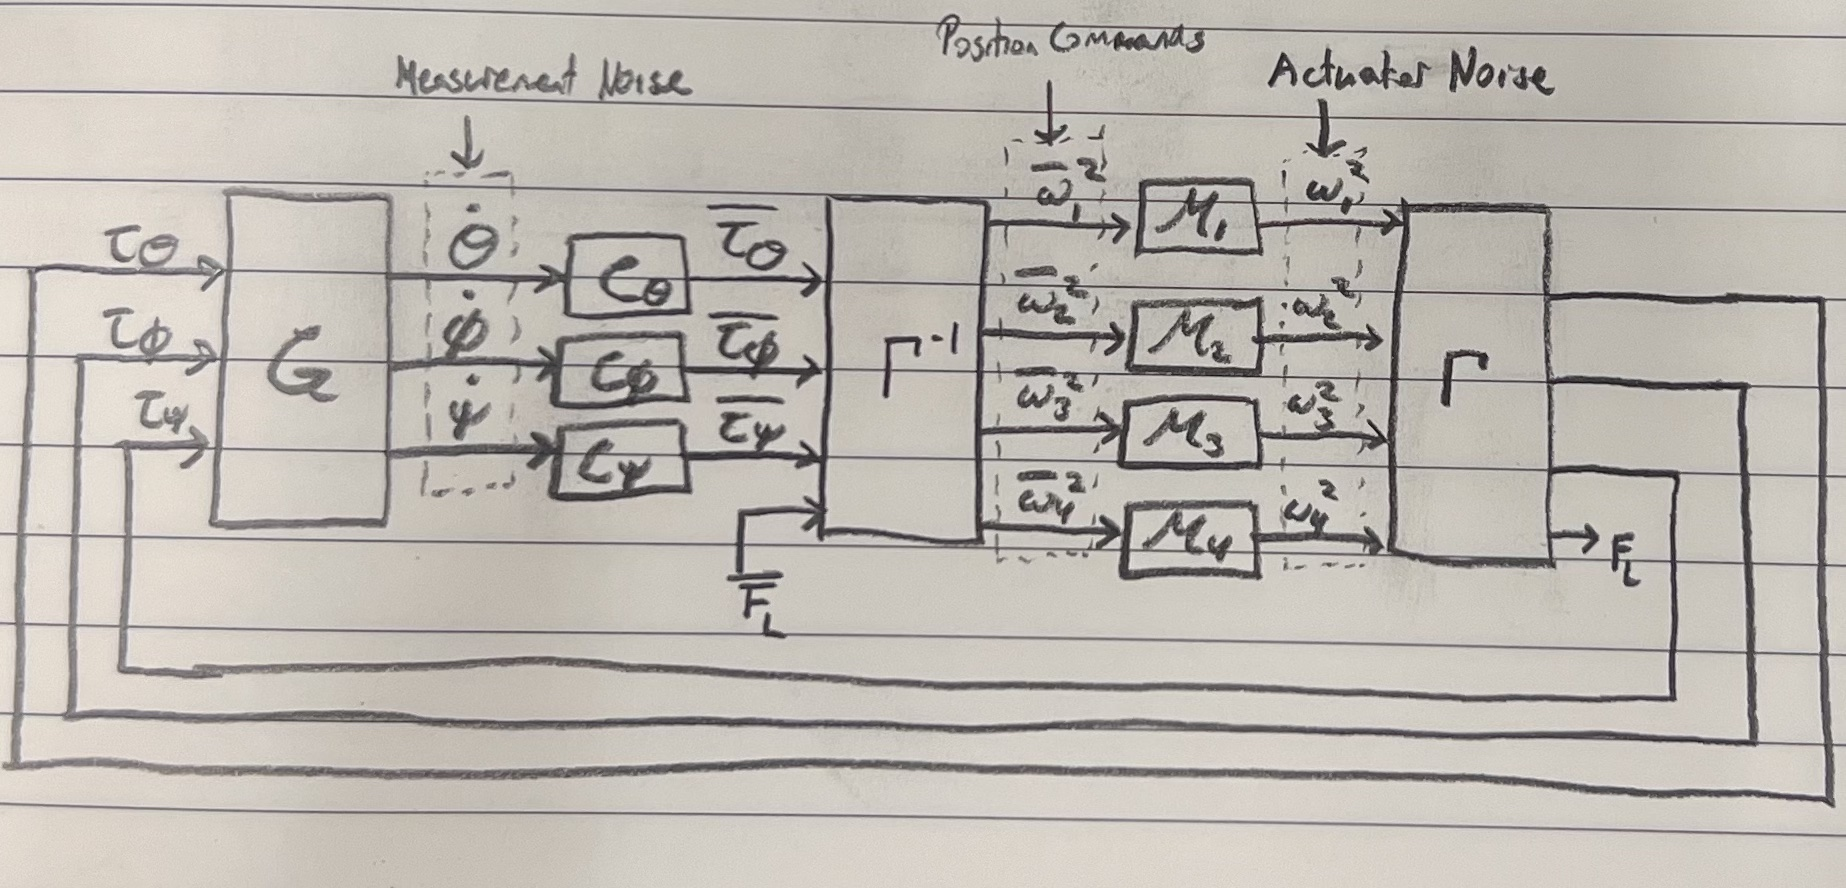
\includegraphics[width=.8\textwidth]{DroneNetwork}
	\caption{Drone decomposed into network with motor dynamics. (Note, where it says ``Measurement noise", ``Position commands", and ``Actuator Noise", it means those exogenous signals are added in those places).} \label{fig:DroneNetwork}
\end{figure}

Now, consider the case where the controllers have access to roll, pitch, and yaw rates as well as the rotor speeds (via back-EMF measurement). Then \autoref{fig:DroneNetwork} looks more like \autoref{fig:DroneNetwork2}.

\begin{figure}
	\centering
	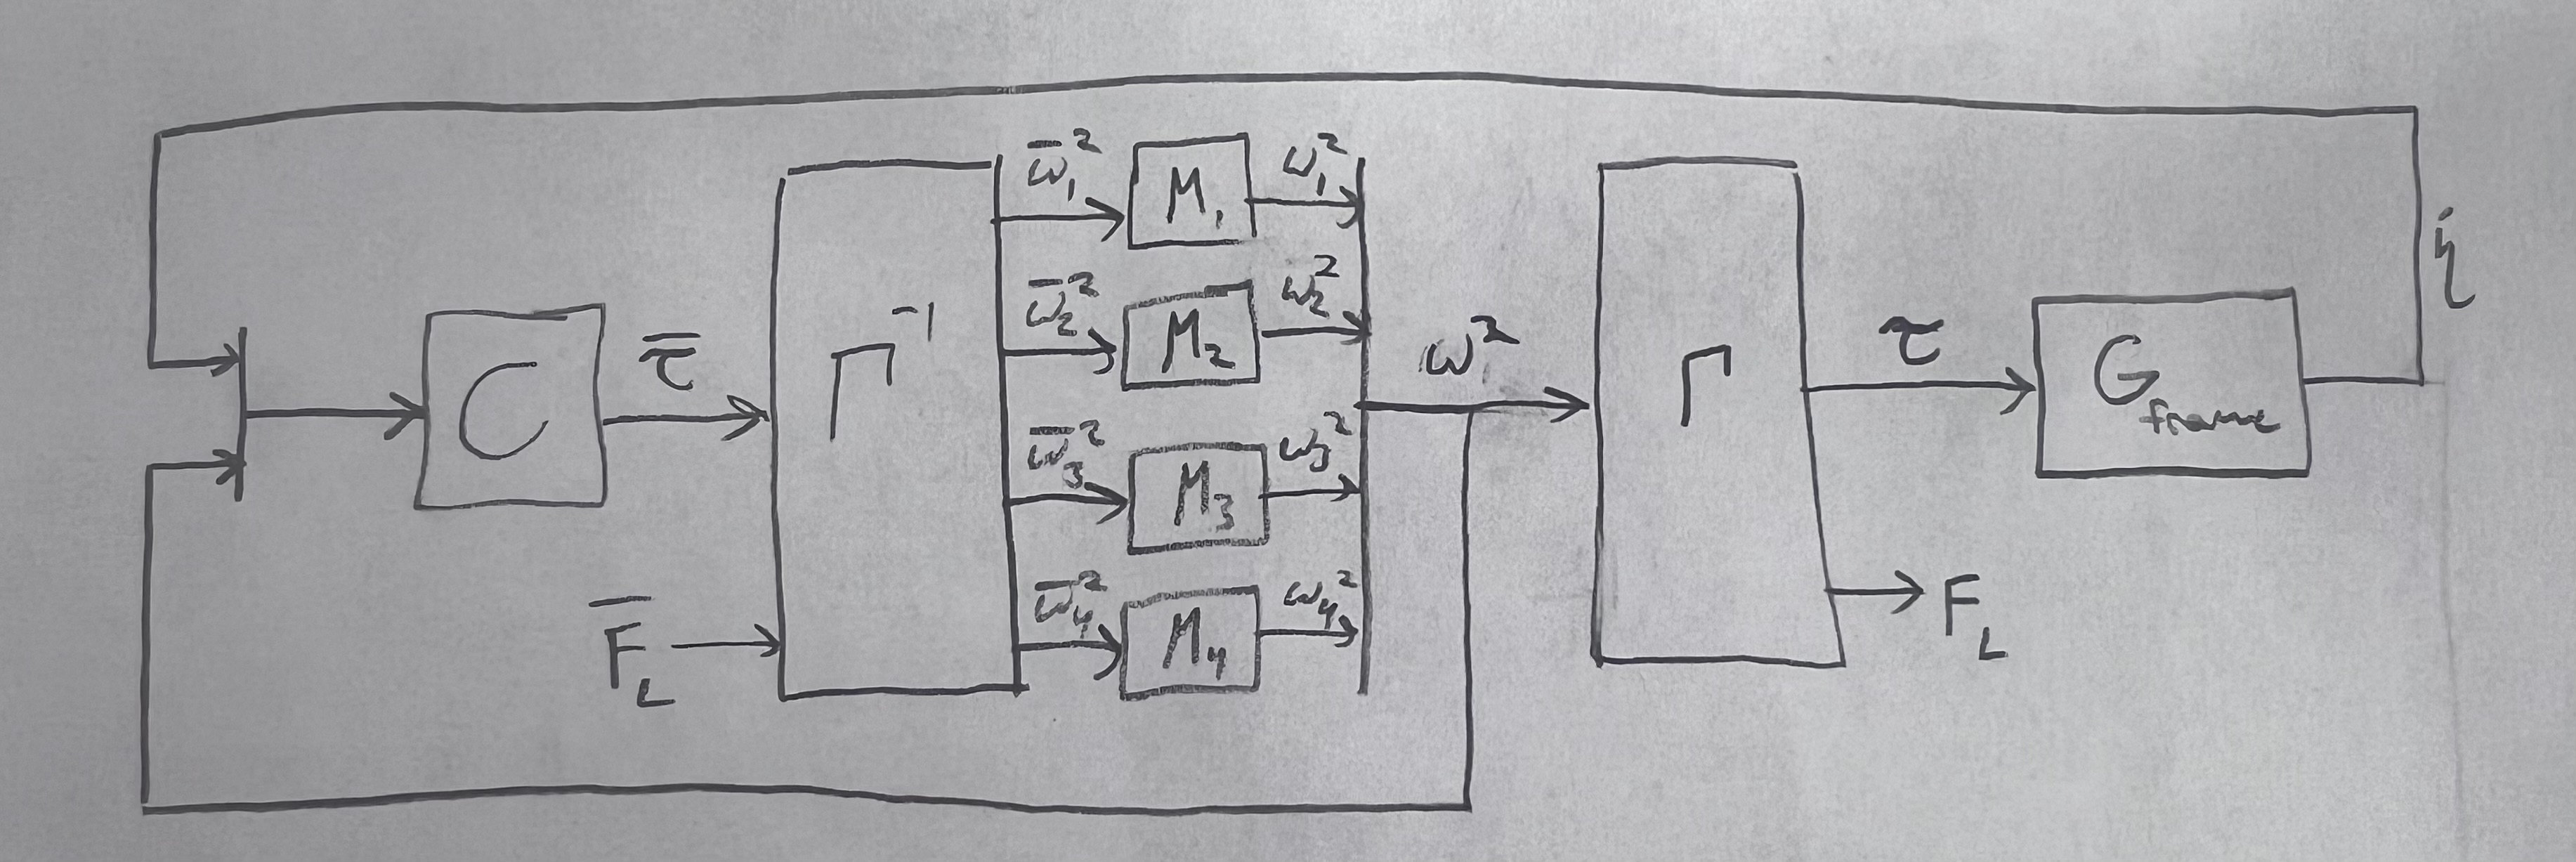
\includegraphics[width=.8\textwidth]{DroneNetwork2}
	\caption{Drone decomposed into network with motor dynamics, with a controller that has access to roll, pitch, yaw rates and rotor speeds.} \label{fig:DroneNetwork2}
\end{figure}

Converting \autoref{fig:DroneNetwork2} into the form for VNDT, we have
\begin{align*}
	G &= \mbox{diag}(G_\mathrm{frame},\, M,\, C) \\
	M &= \mbox{diag}(M_1,\,M_2,\,M_3,\,M_4) \\
	\eta&= \bmat{\theta \\ \phi \\ \psi}, \qquad y = \bmat{\dot{\eta} \\ \omega^2 \\ \overline{\tau}}, \qquad u = \bmat{\tau \\ \overline{\omega}^2 \\ \dot{\eta} \\ \omega^2} \qquad  \tau = \bmat{\tau_\theta \\ \tau_\phi \\ \tau_\psi} \qquad \omega = \bmat{\omega_1 \\ \omega_2 \\ \omega_3 \\ \omega_4}\\
	H &= \bmat{0 & \Gamma_0 & 0 \\ 0 & 0 & \Gamma_0^{-1} \\ I_3 & 0 & 0 \\ 0 & I_4 & 0} \\
	\Gamma_0 &= \bmat{0 & lk & 0 & -lk \\ lk & 0 & -lk & 0 \\ -b & b & -b & b}, \Gamma_0^{-1} = \bmat{0 & \frac{1}{2lk} & -\frac{1}{4b} \\ \frac{1}{2lk} & 0 & \frac{1}{4b} \\ 0 & -\frac{1}{2lk} & -\frac{1}{4b} \\ -\frac{1}{2lk} & 0 & \frac{1}{4b}} \\
	Q &= \bmat{Q_f & 0 & 0 \\ 0 & Q_M & 0 \\ 0 & 0 & Q_C} \\
	S &= \bmat{S_f & 0 & 0 & 0 \\ 0 & S_M & 0 & 0 \\ 0 & 0 & S_c^1 & S_c^2} \\
	R &= \bmat{R_f & 0 & 0 & 0 \\ 0 & R_M & 0 & 0 \\ 0 & 0 & R_c^{11} & R_c^{12} \\ 0 & 0 & R_c^{{12}^T} & R_c^{22}} \\
	SH &= \bmat{0 & S_f\Gamma_0 & 0 \\ 0 & 0 & S_M\Gamma_0^{-1} \\ S_c^1 & S_c^2 & 0} \\
	H^TRH &= \bmat{R_c^{11} & R_c^{12} & 0 \\ R_c^{{12}^T} & R_c^{22} + \Gamma_0^TR_f\Gamma_0 & 0 \\ 0 & 0 & \Gamma_0^{-T}R_M\Gamma_0^{-1}} \\
	\overline{Q} &= Q + SH + H^TS^T + H^TRH = \bmat{Q_f + R_c^{11} & S_f\Gamma_0 + R_c^{12} & S_c^{1^T} \\ * & Q_M + R_c^{22} + \Gamma_0^TR_f\Gamma_0 & S_M\Gamma_0^{-1} + S_c^{2^T} \\ * & * & Q_c + \Gamma_0^{-T}R_M\Gamma_0^{-1}}.
\end{align*}
How did we get that? First, we pick the order of systems: frame, then motors, then controller. We pick the inputs and outputs correspondingly. Then to get $H$, we use the formula $u = Hy$. So the each $u$ component should be some linear combination of the $y$ components. For the first, $\tau = \Gamma_0\omega^2$, which is $u_1 = \Gamma_0y_2$. The idea of $\Gamma_0$ ($\Gamma_0^{-1}$) is that it removes the row (column) that corresponds to the lift force, which is not currently incorporated in the controller or frame dynamics, since we're just working on attitude control.  Repeating this process for each component of $u$ yields $H$. The dimensions of $Q_c$, $S_c$, and $R_c$ are a little tricky, due to the double feedback to $C$ from different parts of the network. Since it has one output, $Q_c$ is blockwise $1\times1$, and $S_c$ has one block row. Since $C$ has two inputs, $S_c$ has two block columns, and $R_c$ is blockwise $2\times 2$. Then applying VNDT gives $\overline{Q}$, which must be negative definite to ensure stability.

The important open question is whether there exists a choice of $Q_c$, $S_c$, and $R_c$ that make $\overline{Q}<0$. Presuming the drone is passive, we have $Q_f = 0$, $S_f = 1$, $R_f = 0$, therefore,
\begin{align*}
	\overline{Q} &=  \bmat{R_c^{11} & \Gamma_0 + R_c^{12} & S_c^{1^T} \\ * & Q_M + R_c^{22}  & S_M\Gamma_0^{-1} + S_c^{2^T} \\ * & * & Q_c + \Gamma_0^{-T}R_M\Gamma_0^{-1}}.
\end{align*}
Immediately, we need $R_c^{11}\leq 0$, which is possible but somewhat concerning. We might be looking at an excone here for the controller. Let's choose $R_c^{12} = -\Gamma_0$, $S_c^{1^T} = 0$, and $S_c^{2^T} = -S_M\Gamma_0^{-1}$, so that we have
\begin{align*}
	\overline{Q} &=  \bmat{R_c^{11} & 0 & 0 \\ * & Q_M + R_c^{22}  & 0 \\ * & * & Q_c + \Gamma_0^{-T}R_M\Gamma_0^{-1}}.
\end{align*}
Now let $R_c^{11} = -\epsilon$, $R_c^{22} = -Q_M-\epsilon$, and $Q_c = -\Gamma_0^{-T}R_M\Gamma_0^{-1} - \epsilon$. Then we have $\overline{Q} = -\epsilon I <0$ (which implies network stability) with
\begin{align}
	\bmat{Q_c & S_c \\ * & R_c} = \bmat{-\Gamma_0^{-T}R_M\Gamma_0^{-1} & 0 & -S_M\Gamma_0^{-1} \\ * & 0 & -\Gamma_0  \\ * & * & -Q_M} - \epsilon I. \label{eqn:ctrlDiss}
\end{align}
The matrix in \autoref{eqn:ctrlDiss} needs to be indefinite or positive definite to be realizable by some controller. Likewise, 
\begin{align*}
	\bmat{Q_M & S_M \\ * & R_M}	
\end{align*}
must be indefinite or positive definite to be realizable. Suppose $Q_M <0$, $R_M >0$, and $S_M = 0$, which satisfies indefiniteness (this is a small gain characterization, which would be easy to find for the motor). Then $-\Gamma_0^{-T}R_M\Gamma_0^{-1} <0$ and $-Q_M>0$, which means $Q_c<0$ and $R_c^{22}>0$. So the controller QSR is indefinite as well. Therefore, if the frame is passive and the motors are gain-bounded, then there is at least one dissipativity characterization of the controllers that makes the network input-output stable!




\end{document}